\documentclass[summaries.tex]{subfiles}
\begin{document}
\section{Ideas}
\subsection{Line search}
Line search in \ref{eqn:update_lsearch} is not working very well. 
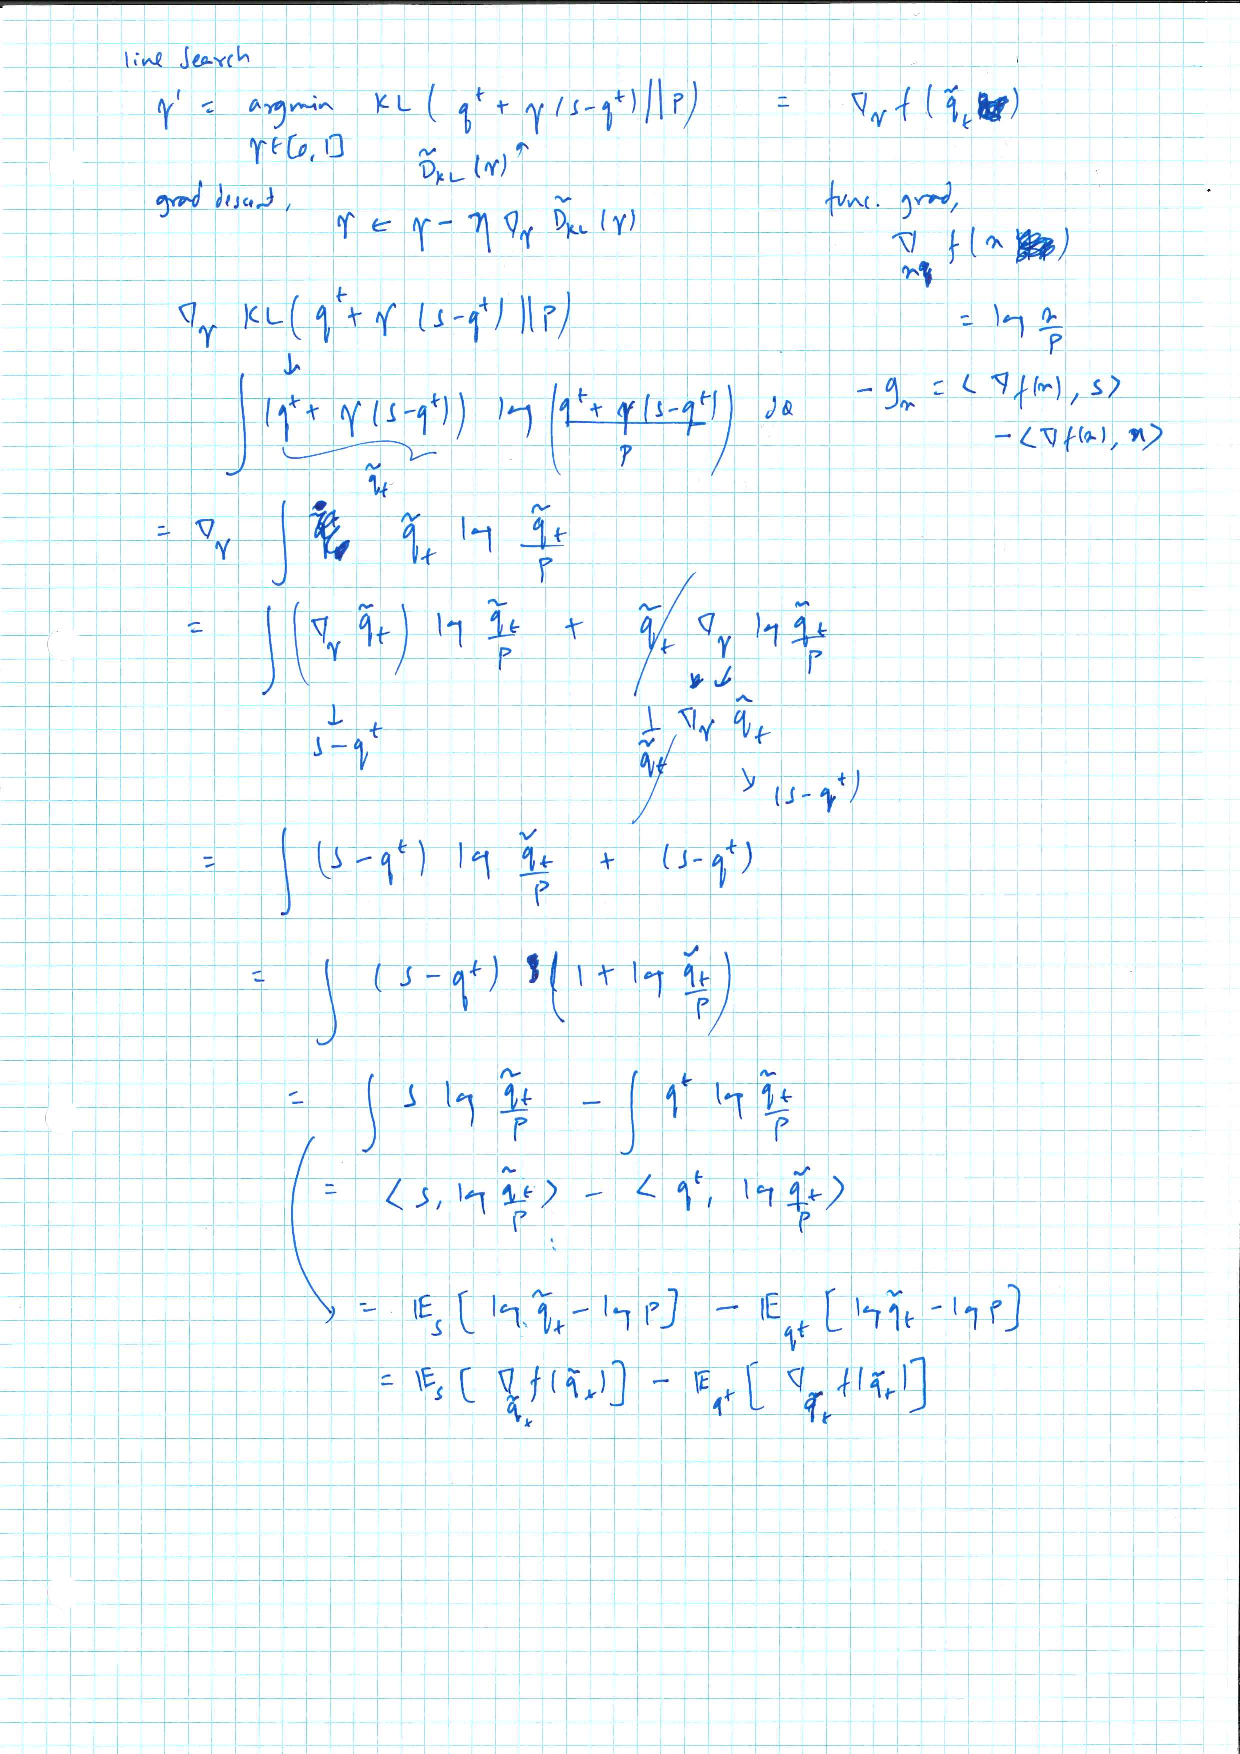
\includepdf{line_search_grad.pdf}
%\inputminted[firstline=140,lastline=220,mathescape]{python}
%  {../boosting_bbvi/scripts/mixture_model_relbo.py}
\mypar{changes for measuring variance of $\EEE{s}{\cdot}$ and $\EEE{q_{t+1}^{\gamma}}{\cdot}$}
\begin{minted}{python}
    ...
    grad_gamma = []
    for it in range(n_steps):
    ...
    # Samples w.r.t s
    rez_s = np.asarray([
        px_qx_ratio_log_prob(sample_s[ss]) for ss in range(len(sample_s))
    ])
    # Samples w.r.t $q_{t+1}$
    rez_q = np.asarray([
        px_qx_ratio_log_prob(sample_q[ss]) for ss in range(len(sample_q))
    ])
    grad_gamma.append({'E_s': rez_s, 'E_q': rez_q, 'gamma': gamma})
    ...
    # Write grad_gamma to outdir/line_search_samples_<n_samples>.npy.<fw_iter>
\end{minted}
\mypar{Metrics on original version}
\begin{figure}[h] \label{fig:gamma}
  \centering
  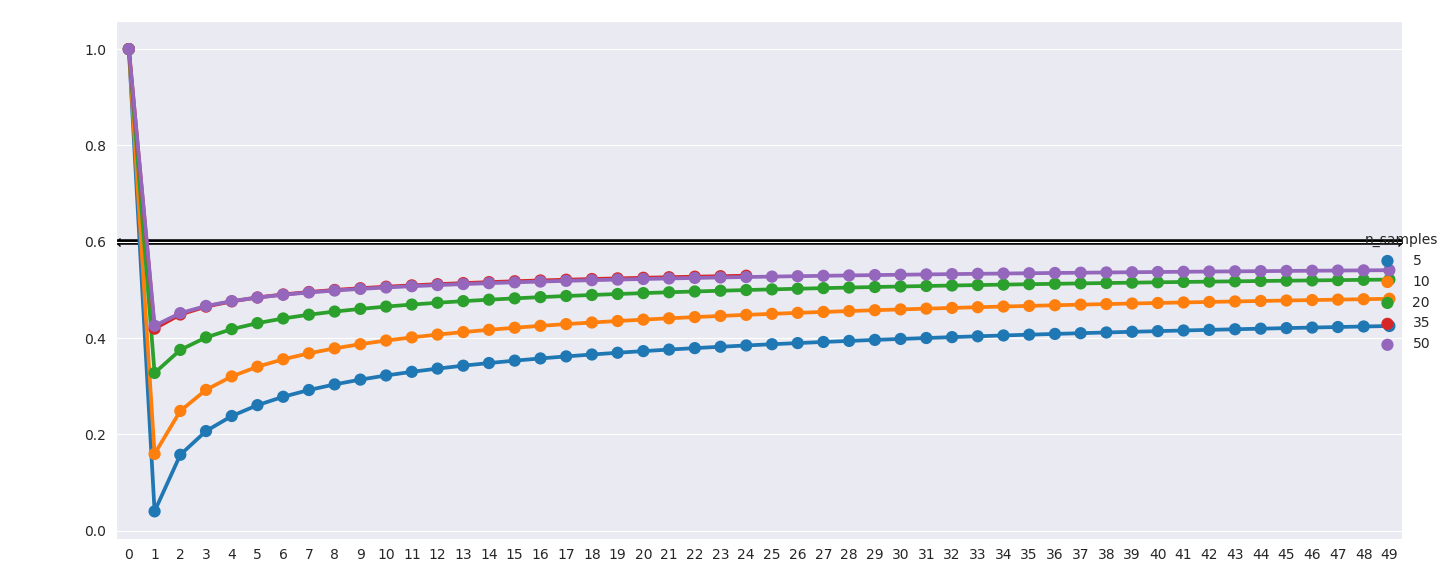
\includegraphics[width=0.9\textwidth]{plots/test_gamma.png}
  \caption{gamma with iterations for different n\_samples}
\end{figure}
\begin{figure}[h] \label{fig:es}
  \centering
  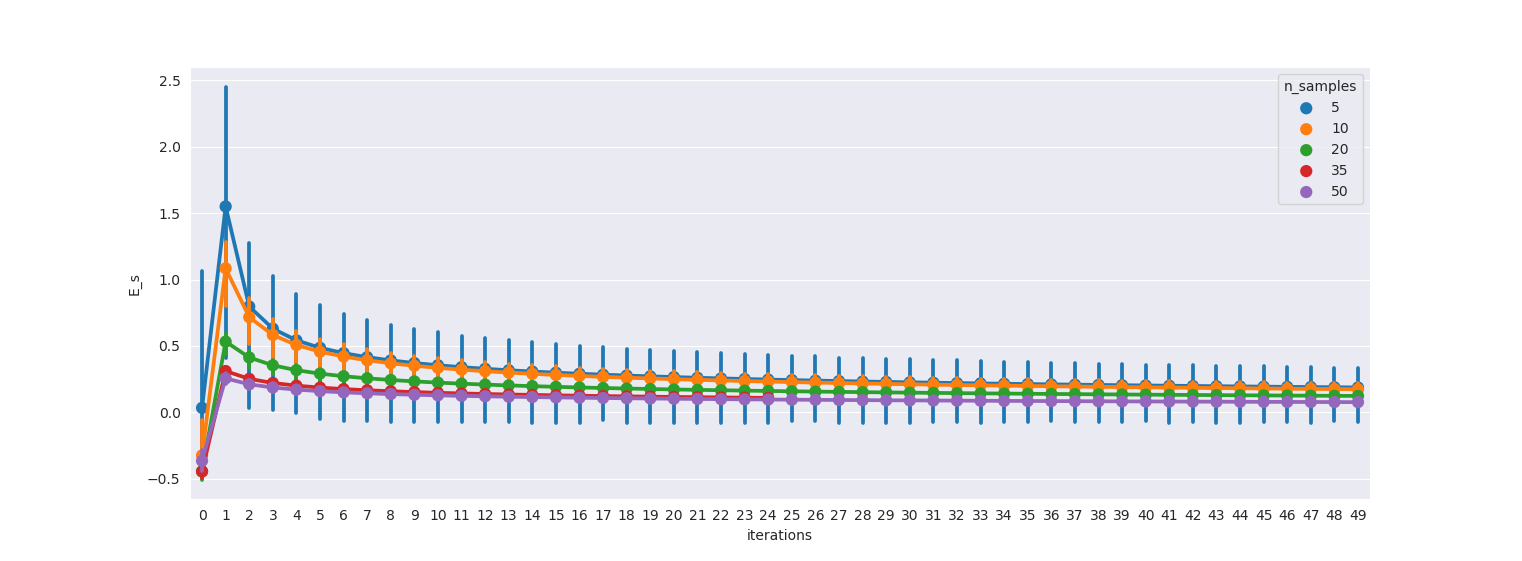
\includegraphics[width=0.9\textwidth]{plots/test_e_s.png}
  \caption{$E_s$ with different n\_samples}
\end{figure}
\begin{figure}[h] \label{fig:eq}
  \centering
  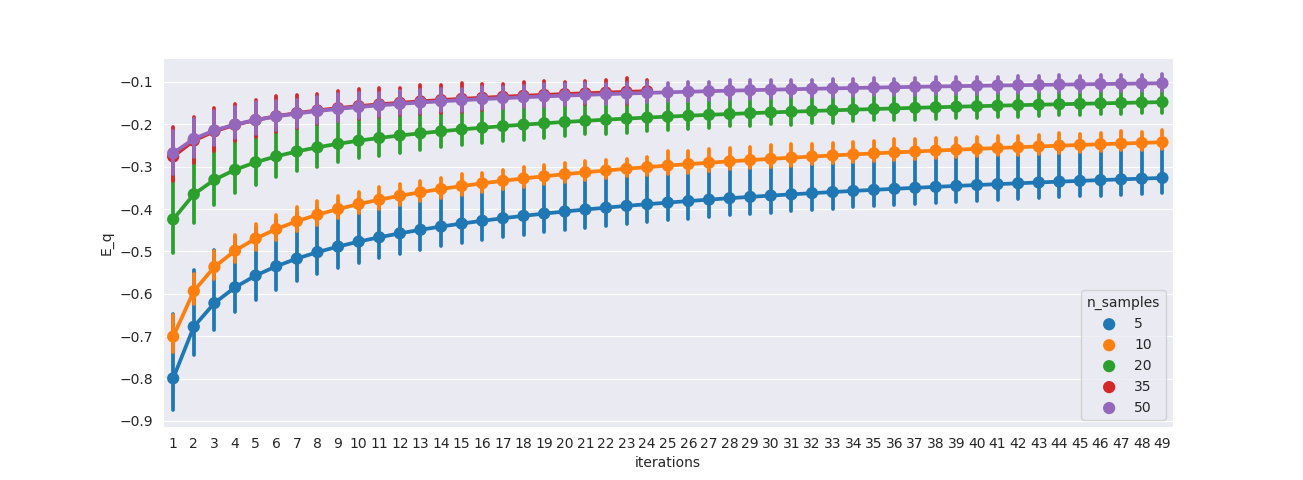
\includegraphics[width=0.9\textwidth]{plots/test_e_q.png}
  \caption{$E_q$ with different n\_samples}
  \small{\comm{\ref{fig:eq} begins with iter 1 as iter 0 has very high variance}}
\end{figure}

\subsection{Adaptive Frank-Wolfe from smoothness estimators}
Algorithm 1 of \cite{pedregosa2018step}
\begin{algorithm}[h]
  \KwIn{$q_0 \in \data$, initial Lipschitz estimate $L_{-1}$, line search parameters
  $\tau > 1, \eta \in (0, 1]$}
  \For{t = 1...T} {
    $s_t \gets LMO_{\family}(\grad f(q^t))$\\
    $g_t \gets \langle \grad f(q_t), q_t \rangle - 
    \langle \grad f(q_t), s_t \rangle$ \tcp{Gap $\geq 0$}\\
    Find smallest integer i s.t\\ {
      $f(q_t + \gamma_t(s_t - q_t)) \leq Q_t(\gamma_t)$ Where\\
      $Q_t(\gamma) := f(q_t) - \gamma g_t + \frac{\gamma^2 L_t}{2}d(s_t, q_t)$
      \tcp{Quadratic upper bound \ref{eqn:quad_upper}}\\
      $L_t \gets \tau^i\eta L_{t-1}$ and
      $\gamma_t \gets \min\Big(\frac{g_t}{L_t d(s_t, q_t)}, 1\Big)$
    }
  }
  \Return{$q_T$}
  \label{alg:adafw}
  \caption{Adaptive Frank-Wolfe for Boosting BBVI}
\end{algorithm}

\mypar{Code changes}

\subsection{Measuring smoothness}
\INPROGRESS
Computing optimal $\gamma$ directly
from eqn 1 of \cite{pedregosa2018step}
\begin{align*}
  f(\bx_{t+1}) &\leq f(\bx_t) + \gamma \langle \grad f(\bx_t), \bs_t - \bx_t \rangle 
  + \frac{\gamma^2}{2}L_t ||\bs_t - \bx_t||^2 \\
  \Rightarrow L_t &\geq \frac{f(\bx_{t+1}) - f(\bx_t) 
  + \gamma \langle \grad f(\bx_t), \bs_t - \bx_t \rangle}
  {\frac{\gamma^2}{2}||\bs_t - \bx_t||^2}  \\
                  &\frac{f(\bx_{t+1}) - f(\bx_t) 
                  + \gamma \langle \grad f(\bx_t), \bs_t - \bx_t \rangle}
                  {\frac{\gamma^2}{2} \red{\kl{s_t || q_t}}}  \\
\end{align*}
\mypar{Code changes}
\begin{minted}{python}
def grad_kl(q, p, theta):
    # Functional Gradient w.r.t q $\nabla KL(q || p) = \log q - \log p$
    ...


def lmo(y, p, ...):
    # $f = \mathcal{D}^{KL}(y || p)$
    # $\langle \nabla f , y \rangle = \mathbb{E}_{y}{\nabla f}$
    ...
\end{minted}

\subsection{Other optimization algorithm}
\TODO
As shown in link \ref{web:cmu}, Frank-Wolfe converges slower than Projected 
Gradient Descent in Practice. See \cite{locatello2017boosting} to see why we use
FW and if it can be replaced. (will have to derive new convergence proofs and
boosting won't be as integrated into the optimization algorithm as before).

\subsection{Entropy Regularization and Noise addition using Optimal Transport}
In LMO, \cite{locatello2018boosting} uses Entropy Regularization in place of
norm constrained optimization. It can be replaced with something simpler 
See \cite{tolstikhin2017wasserstein} \cite{liu2018entropy} \cite{bernton2017inference}
\cite{jordan1998variational} \href{https://www-dimat.unipv.it/savare/Ravello2010/JKO.pdf}
{here} And \cite{peyre2017computational} part 4.

\subsection{Port code to Tensorflow Probability}
see \ref{code:ed_tf_issue}. Issue is if \texttt{tfp.edward2} will have support
for Variational Inference and ELBO etc.

\biblio
\end{document}
